\documentclass{beamer}
\usepackage{animate}
\usepackage{multimedia}
\usepackage[english,russian]{babel}

\usepackage{pgfpages}
\setbeameroption{show notes on second screen}
%https://tug.ctan.org/macros/latex/contrib/beamer/doc/beameruserguide.pdf

\usepackage[T2A]{fontenc}
\usepackage[utf8]{inputenc}

\setbeamertemplate{caption}[numbered]

\usetheme{CambridgeUS}
\usecolortheme{dolphin}


\title[Радиометрия]{Радиометрия и оптика}
\author[Быковских Д.А.]{Быковских Дмитрий Александрович}
\date{16.12.2023}

\begin{document}
	\begin{frame}
		\titlepage
	\end{frame}
	% \begin{frame}{Содержание}
	% \end{frame}
	%\section{Обзор}
	\begin{frame}{Введение}
		Оптика --- это раздел физики, изучающий свет и его взаимодействие с веществом, а также явления, связанные с распространением света, его преломлением, отражением, дифракцией и интерференцией.

		Радиометрия --- это наука о измерении электромагнитного излучения в различных частях спектра, включая видимую световую область, инфракрасное и ультрафиолетовое излучение, радиоволны и другие формы излучения. Радиометрия описывает количественные характеристики излучения, такие как поток энергии, интенсивность и яркость, и используется в различных областях, включая астрономию, фотометрию и измерения теплового излучения.
	\end{frame}

	\begin{frame}{Геометрическая модель} %{Энергетические единицы}

		В оптике энергия излучения определяется за время на много больше, чем период собственных колебаний электромагнитных волн оптического диапазона ($10^14$ Гц).

		Рассматривается простая геометрическая модель, являющаяся следствием уравнения Максвелла, согласно которой
		свет представляет собой поток лучистой энергии, распространяющийся вдоль геометрических лучей.

		Электромагнитное поле в однородных изотропных средах переносит энергию $E$ в направлении, которое указывается оптическим лучевым вектором $q$.

		Энергия измеряется в джоулях Дж.

		Поток излучения (лучистый поток) ---  это величина энергии, переносимой полем в единицу времени через данную площадку.

		$\Phi_e = \frac{E}{t} = \frac{\text{Дж}}{\text{с}} = \text{Вт}$

		\note{
			% http://aco.ifmo.ru/el_books/basics_optics/glava-2/glava-2-1.html
			\begin{figure}
				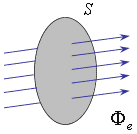
\includegraphics[width=0.45\textwidth]{images/image410.png}
				\caption{Поток излучения}
			\end{figure}
		}

	\end{frame}

	\begin{frame}{Геометрическая модель}
		Поверхностная плотность потока энергии $E_e$ --- величина потока $\Phi_e$, приходящаяся на единицу площади $S$.
		\[
			E_e = \frac{\partial \Phi_e}{\partial S}, \qquad \bigg[ \frac{\text{Вт}}{\text{м}^2} \bigg]
		\]
		Но также может быть наоборот.
		
		$M_e$ --- энергетическая светимость.

		Если поток излучается площадкой, то поверхностная плотность потока энергии будет иметь смысл энергетической светимости.

		\note{

			\[
				\int E_e d S = \Phi_e
			\]
			\[
				\int \int E_e d x d y = \Phi_e
			\]
		}
	\end{frame}



	\begin{frame}{Телесный угол}{Solid angle}

		Телесный угол $\Omega$ (или твердый угол) представляет собой меру пространственного угла, измеряемого в трехмерном пространстве. Он определяется как соотношение площади проекции поверхности, заключенной между лучами, выпущенными из точки и пересекающими какой-то объект (обычно сферу), к квадрату радиуса этой сферы. Таким образом, телесный угол измеряет, насколько много пространства охватывает объект относительно точки наблюдения. Его единицей измерения является стерадиан (ср).
		\note{
			\begin{figure}
				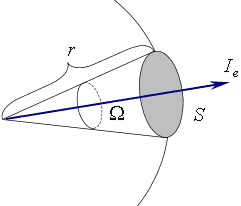
\includegraphics[width=0.45\textwidth]{images/image696.png}
				\caption{Телесный угол}
			\end{figure}
		}

	\end{frame}

	\begin{frame}{Угол и телесный угол}{Angle and Solid Angle}

		Рассмотрим следующие формулы
		\[
			d \theta = \frac{d L}{r}	
		,
		\]
		где
		\(d\theta\) --- изменение угла \(\theta\);
		\(dL\) --- изменение длины дуги;
		\(r\) --- радиус сферических координат.
		

		Следующая формула используется при интегрировании по сферической поверхности и является результатом преобразования элемента поверхности \(dS\) в сферических координатах.
		\[
			d \Omega = \frac{dS}{r^2} 
			= 
			\frac{(r d \phi)(r \sin \theta d \theta)}{r^2} 
			= 
			\sin \theta  d \theta d \phi
			,
		\]
		где
		\(d\Omega\) --- элемент телесного угла;
		\(dS\) --- элемент поверхности;
		\(r\) --- радиус сферических координат;
		\(d\theta\) --- элемент угла \(\theta\) (зенитного угла);
		\(d\phi\) --- элемент угла \(\phi\) (азимутального угла).
		

		\note{
			\begin{figure}
				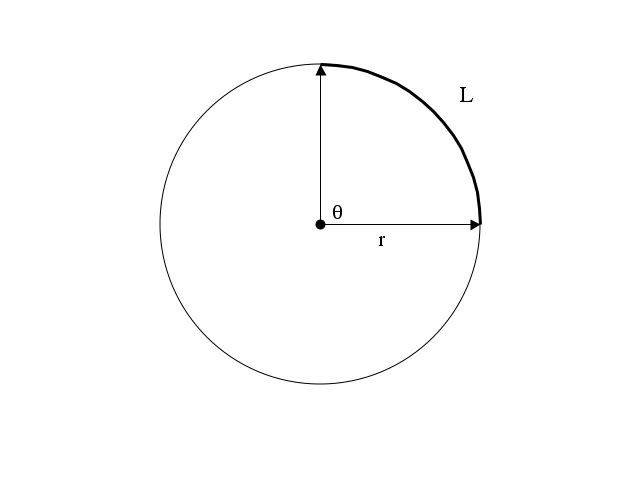
\includegraphics[width=0.45\textwidth]{images/radians.jpg}
				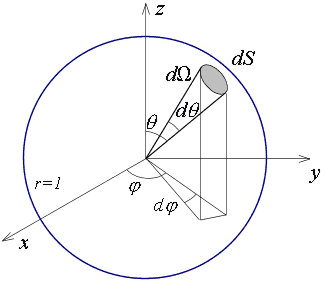
\includegraphics[width=0.45\textwidth]{images/solid_angle_2.png}
				\caption{Угол в полярных координатах и телесный угол в сферических координатах}
			\end{figure}
		}
	\end{frame}

	\begin{frame}{Площадь сферы}{Differential Solid Angles}
		Итак, телесный угол описывается следующей формулой
		\[
			d \omega = \frac{d S}{ r^2} =	\sin \theta  d \theta d \phi
		\]
		Площадь единичной сферы через телесный угол и в сферической системе координат
		\[
			\Omega = \int_{S} d \omega 
			= 
			\int_{0}^{2\pi}\int_{0}^{\pi} \sin \theta  d \theta d \phi
			= 
			\int_{0}^{\pi} \sin \theta d \theta \int_{0}^{2\pi} d \phi
			=
			4 \pi
		\]

		\note{
			\begin{figure}
				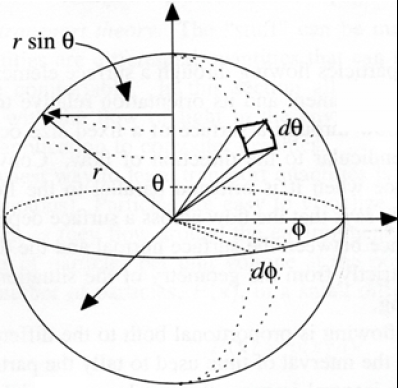
\includegraphics[width=0.55\textwidth]{images/sphere_surface.png}
				\caption{Схема расчета сферы}
			\end{figure}
		}
	\end{frame}

	\begin{frame}{Ракурс}{Foreshortening}
		Большой источник, рассмотренный под косым углом, должен создавать тот же эффект, что и маленький источник, расположенный перпендикулярно. Это явление известно как ракурс.

		\note{
			\begin{figure}
				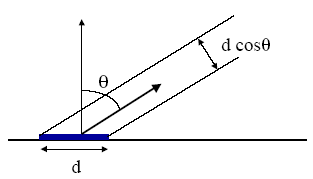
\includegraphics[width=0.75\textwidth]{images/foreshortening.png}
				\caption{Ракурс}
			\end{figure}
		}
	\end{frame}
	
	\begin{frame}{Телесный угол}{Solid Angle}
		
		Телесный угол $\omega$ определяется проектируемой площадью поверхности на единичную сферу от точки.

		Телесный угол образуется точкой и участком поверхности.

		\[
			d \omega = d A_0 = \frac{d A \cos \theta}{ r^2}
		\]

		\note{
			\begin{figure}
				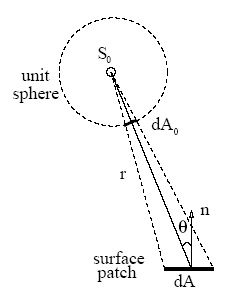
\includegraphics[width=0.4\textwidth]{images/solid_angle_.png}
				\caption{Телесный угол}
			\end{figure}
		}
	\end{frame}



	\begin{frame}{Излучение}{Radiance}
		Распределение света в пространстве зависит от положения и направления. Подходящей единицей измерения для оценки распределения света в пространстве является радианс, который определяется как мощность (количество энергии в единицу времени), перемещающаяся в какой-то точке в определенном направлении, на единицу площади, перпендикулярной направлению движения, на единицу телесного угла. Кратко говоря, радианс представляет собой количество света, излучаемого из точки... (в единичный телесный угол, с единичной площади).

		% Radiance = Power / (solid angle x foreshortened area)
		% W/sr/m2
		% W is Watt, sr is steradian, m2 is meter-squared

		\note{
			
			\begin{figure}
				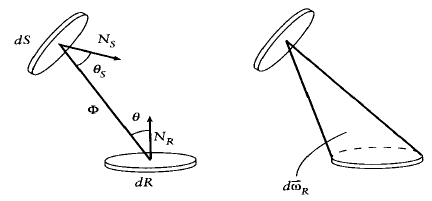
\includegraphics[width=0.9\textwidth]{images/radiance_ds_dr.png}
				\caption{Излучение из ds в dr}
			\end{figure}
		}

	\end{frame}

	\begin{frame}{}
		Формулы энергетической яркости поверхности в конкретном направлении
		% \[
		% 	I = \frac{\Phi}{d \omega}
		% \] 
		\[
			L = \frac{d^2 \Phi}{\cos \theta d \omega d A}
		\] 
		\[
			L \cos \theta d \omega = \frac{d^2 \Phi}{ d A}
		\] 
		где 
		$L$ --- энергетическая яркость (Radiance), описывает количество светового потока, излучаемого поверхностью в определенном направлении, на единичную площадку и в единичный угловой диапазон ($W/(m²\cdot sr)$);
		$d^2 \Phi$ --- элемент светового потока (Flux) через малую площадку $dA$  в малом угловом диапазоне $d \omega$;
		$\cos \theta$ --- косинус угла между нормалью к поверхности и направлением, в котором измеряется энергетическая яркость;
		$dA$ --- элемент площади поверхности, через которую измеряется световой поток;
		$d \omega$ --- элемент углового диапазона, в пределах которого измеряется световой поток.
		
	\end{frame}

	\begin{frame}{Бесконечно маленький источник света и участки поверхности}

		Radiance at x1 leaving to x2
		\[
			L(x_1,x_1 \to x_2) = 
			\frac{d \Phi}{d \omega \cos \theta_1 d A_1}
			=
			\biggl[ 
				d \omega = \frac{\cos \theta_2 d A_2 }{ r^2}
			\biggr]
			=
			\frac{r^2 d \Phi}{\cos \theta_2 d A_2   \cos \theta_1 d A_1}
		\]

		Let the radiance arriving at x2 from the direction of x1 is

		\[
			L(x_2,x_1 \to x_2) = 
			\frac{d \Phi}{d \omega \cos \theta_2 d A_2}
			=
			\biggl[ 
				d \omega = \frac{\cos \theta_1 d A_1 }{ r^2}
			\biggr]
			=
			\frac{r^2 d \Phi}{\cos \theta_1 d A_1 \cos \theta_2 d A_2}
		\]

		\note{
			
		\begin{figure}
			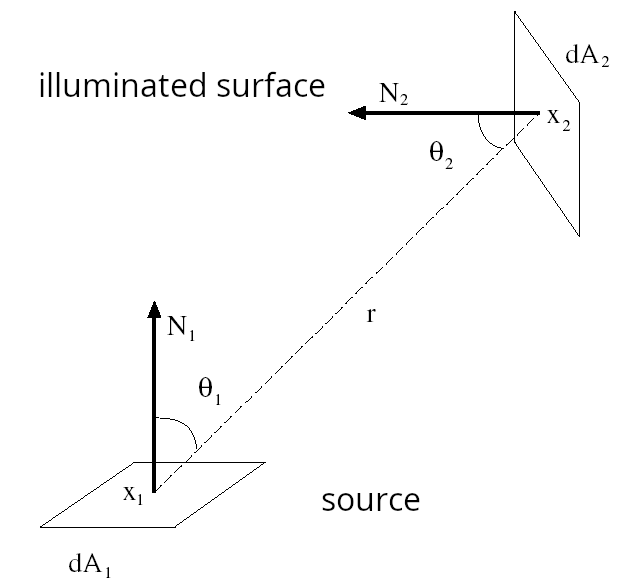
\includegraphics[width=0.6\textwidth]{images/radiance_ds_dr_.png}
			\caption{Излучение из ds в dr}
		\end{figure}
		}
	\end{frame}

	\begin{frame}{Расчет излученной энергии}{Computing Irradiance}
		
	Интегрируйте световой поток по полусфере
		\[
			E(x) = \int_{\Omega} L(x, \theta_i, \phi_i) \cos \theta_i d \omega
			=
			\int_{0}^{2\pi}\int_{0}^{\pi / 2} 
			L(x, \theta_i, \phi_i) 
			\cos \theta_i \sin \theta_i d \theta d \phi
		\]
	Таким образом, излученная энергия из определенного направления составляет

	\[
		E(x) = L(x, \theta_i, \phi_i) \cos \theta_i d \omega
	\]

	\end{frame}

	\begin{frame}{Двулучевая функция отражательной способности}{Bidirectional Reflectance Distribution Function, BRDF}
		
		Двулучевая функция отражательной способности (ДФОС) описывает какая доля световой энергии, приходящей из одного направления, уходит в другом направлении для произвольной пары таких направлений. 
		
		Математически выражается следующим образом:
		% \[ \text{BRDF}(\theta_o, \phi_o, \theta_i, \phi_i) = \frac{\text{Исходящая яркость}(\theta_o, \phi_o)}{\text{Входящая интенсивность}(\theta_i, \phi_i)} \]
		% или

		\[
			%\text{BRDF}
			f_r
			(\theta_o, \phi_o, \theta_i, \phi_i) =
			% f(\theta_o, \phi_o,\theta_i, \phi_i) =
			\frac{d L(\theta_o, \phi_o)}{d E (\theta_i, \phi_i)}
			% переписать знаменатель через L cos d w
		\]


		Здесь \(\theta_i\) и \(\phi_i\) представляют углы направления входящего света (обычно относительно нормали к поверхности), а \(\theta_o\) и \(\phi_o\) представляют углы направления исходящего света. 

		BRDF является фундаментальным концептом,
		% в компьютерной графике, компьютерном зрении и оптике, 
		предоставляя способ моделирования взаимодействия света с поверхностями и его отражения в различных направлениях.

		\note{
		\begin{figure}
			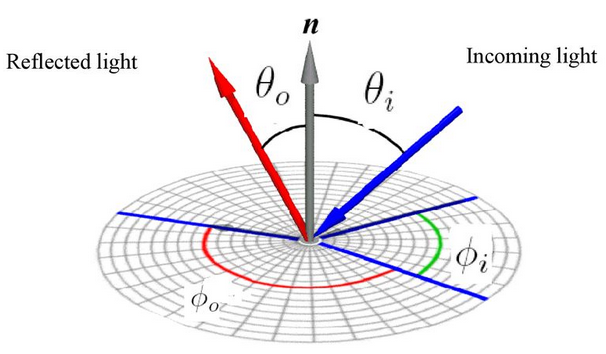
\includegraphics[width=0.8\textwidth]{images/brdf_2.png}
			\caption{Двулучевая функция отражательной способности}
		\end{figure}
		}
	\end{frame}

	\begin{frame}{}
		Излученность в направлении наблюдения при условии всех входящих световых потоков. 
		\[
			L(x, \theta_o, \phi_o) = 
			\int_{\Omega} 
			%\text{BRDF}
			f_r(\theta_o, \phi_o, \theta_i, \phi_i) 
			L(x, \theta_i, \phi_i) 
			\cos \theta_i d \omega
		\]
		Что пропорционально яркости пикселя для этого луча.

		\note{ 
			\footnotesize
			Функция двустороннего распределения отраженного света (BRDF) обладает несколькими важными свойствами:

			1. Положительность: Значения BRDF обычно неотрицательны для всех углов входа и выхода света.
			
			2. Нормализация: Интеграл BRDF по всем направлениям входа и выхода света равен единице. Это свойство обеспечивает сохранение энергии в системе.
			
			3. Ротационная инвариантность: BRDF не зависит от ориентации координатной системы, т.е. она инвариантна относительно поворотов.
			
			4. Симметрия: BRDF симметрична относительно обмена направлений входа и выхода света (\(\theta_i, \phi_i\) и \(\theta_o, \phi_o\)).
			
			5. Локальная изотропия или анизотропия: BRDF может быть изотропной (не зависит от направления) или анизотропной (зависит от направления).
			
			6. Монотонность: Поверхности с монотонной BRDF не могут сосредотачивать свет.
			
			7. Микрогеометрическая зависимость: BRDF часто зависит от микрогеометрии поверхности (например, шероховатости или микронеровностей).
			
			% Эти свойства обеспечивают физически обоснованное и адекватное моделирование отражательных свойств различных материалов в компьютерной графике и графическом дизайне.

		}
	\end{frame}

	\begin{frame}{Световые и энергетические величины}
		\begin{table}
			\caption{\label{tab:fractal} Сравнение энергетических и световых величин}
			\begin{center}
				\renewcommand{\arraystretch}{1.5} 
				\begin{tabular}{|c|c|c|c|c|c|}
					\hline
					\multicolumn{3}{|c|} {Энергетические} & \multicolumn{3}{|c|} {Световые} \\
					\hline
					Поток излучения & $\Phi_e$ & Вт & Световой поток & $\Phi$ & лм \\
					\hline
					Энергетическая сила света & $I_e$ & $\frac{\text{Вт}}{\text{ср}}$ & Сила света & $I$ & кд \\
					\hline
					Энергетическая освещенность & $E_e$ & $\frac{\text{Вт}}{\text{м}^2}$ & Освещенность & $E$ & лк \\
					\hline
					Энергетическая светимость & $M_e$ & $\frac{\text{Вт}}{\text{м}^2}$ & Светимость & $M$ & $\frac{\text{лм}}{\text{м}^2}$ \\
					\hline
					Энергетическая яркость & $L_e$ & $\frac{\text{Вт}}{\text{cр м}^2}$ & Яркость & $L$ & $\frac{\text{кд}}{\text{м}^2}$ \\
					\hline
				\end{tabular}
			\end{center}
		\end{table}

		Примечание.
		Световой поток измеряется в лм (люменах) и представляет собой полную видимую энергию, излучаемую источником света за единицу времени.

		\note{

		Люмен (лм): Люмен измеряет световой поток, представляя собой общее количество света, излучаемого источником света в одну секунду; используется для оценки яркости светильников и ламп.

		Кандела (кд): Кандела измеряет световой поток в заданном направлении, представляя собой интенсивность света в конкретном угловом направлении; введена для оценки яркости источников света, особенно в направленных световых системах.

		Люкс (лк): Люкс измеряет освещенность, представляя собой количество света, падающего на поверхность в один люкс, равный одному люмену на квадратный метр; введен как метрика для оценки комфортного освещения.
		
		Историческая справка. 
		Люкс и лм стали стандартами измерения света в 20 веке, с развитием технологий освещения. В 1948 году была введена спецификация лм для измерения светового потока. Кандела была предложена в 1946 году в ходе разработки стандартов единиц измерения света, утвержденных в 1979 году.
		% https://novolampa.ru/baza-znaniy/kandely-lyuminy-lyuksy-v-chem-raznitsa/

		}
		
	\end{frame}

	\begin{frame}{Освещенность и светимость}
		Освещенность и светимость - это два различных понятия, связанных с освещением, но имеющих разные значения.

    Освещенность: \\
        Определение: Освещенность (или освещенностный поток) измеряет количество света, падающего на единичную поверхность. Единицей измерения освещенности в системе СИ является люкс (лм/м²). \\
        Формула: Освещенность ($E$) = световой поток ($\Phi$) / площадь поверхности ($A$). \\
        Пример: Если у вас есть лампа мощностью 1000 люмен и она освещает поверхность в 10 квадратных метрах, то освещенность будет 100 люкс.

				\note {
				Светимость: \\
						Определение: Светимость относится к общему количеству энергии, излучаемой световым источником во всех направлениях. Единицей измерения светимости в системе СИ является люмен (лм). \\        
						Формула: Светимость ($M$) - это сумма светового потока во всех направлениях.\\         
						Пример: Если у вас есть лампа, излучающая свет во все стороны, и ее световой поток составляет 1000 люмен, то ее светимость также будет 1000 люмен.
		
					Таким образом, освещенность измеряет количество света на единицу площади, в то время как светимость представляет собой общее количество излучаемого света и измеряется в люменах.

				}
		
	\end{frame}

	\begin{frame}{Заключение}
		Литература
		\begin{enumerate}
			\item \href{https://www.ece.lsu.edu/gunturk/EE4780/EE4780.html}{Bahadir K. Gunturk Radiometry, photometric stereo}
			\item \href{http://aco.ifmo.ru/el_books/basics_optics/glava-2/glava-2-1.html}{Родионов С.А. Основы оптики. Конспект лекций}
			\item Jinxiang C. Computer Graphics: Radiometry and Illumination 
			\item \href{https://novolampa.ru/baza-znaniy/kandely-lyuminy-lyuksy-v-chem-raznitsa}{Взаимосвязь силы света, светового потока и освещенности}
		\end{enumerate}

	\end{frame}
	
\end{document}